\chapter{Airship Sequence}

\vspace{\baselineskip}

\begin{paracol}{2}

\begin{enumerate}
    \item Fly to the Ancient Ruins
\end{enumerate}

\switchcolumn
\begin{misc}{Path to the Ancient Ruins}
    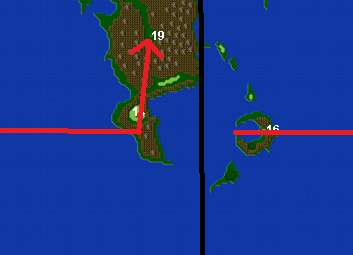
\includegraphics[scale=0.7]{../Graphics/Maps/5. To Ruins.png}
\end{misc}

\switchcolumn
\resume
\begin{enumerate}[resume]
    \item Fly back to Crescent HQ and talk to Cid
\end{enumerate}

\switchcolumnTwice[*]
\newpage
\begin{enumerate}[resume]
    \item Fly to the Tycoon Meteor, stopping at the following island along the way
\end{enumerate}

\switchcolumn
\begin{misc}{Path to the Tycoon Meteor}
    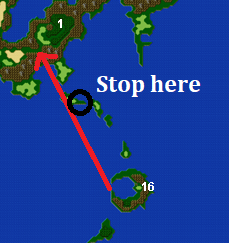
\includegraphics[scale=1.45]{../Graphics/Maps/6. To Tycoon Meteor.png}
\end{misc}

\begin{steproute}{Black Flame x5 Encounters}
    \insertStep{../Graphics/Steps/70. Airship 1.jpg}
    \insertStep{../Graphics/Steps/71. Airship 2.jpg}
\end{steproute}

\switchcolumn
\begin{encounter}{Black Flame x5}
	\varwb
	\begin{notes}
		\item \encounterHl{Hold A entering the encounter}
	\end{notes}
	\begin{round}{1}
		\faris \leftCommand{\throw} \then \thunderScroll
	\end{round}
	\varwe
\end{encounter}

\begin{menu}{After the First Black Flame Encounter}
    \varwb
    \begin{jobMenu}
        \galuf Thief \textbf{(2\pointRight)} \ability{!\white}
        \bartz Bard \textbf{(\pointUp)}
    \end{jobMenu}
    \varwe
\end{menu}

\begin{encounter}{Black Flame x5 (x2)}
	\varwb
	\begin{notes}
		\item \encounterHl{Hold A entering the encounters}
	\end{notes}
	\begin{round}{1}
		\faris \leftCommand{\throw} \then \thunderScroll
	\end{round}
	\varwe
\end{encounter}

\switchcolumn*
\begin{steproute}{After the Encounters}
    \insertStep{../Graphics/Steps/72. Airship 3.jpg}
\end{steproute}

\switchcolumn
\begin{enumerate}[resume]
    \item At the Tycoon Meteor, grab the hidden \pickup{Phoenix Down} on the right
\end{enumerate}

\begin{menu}{Before Adamantoise}
    \varwb
    \begin{jobMenu}
        \bartz Blue Mage \textbf{(\pointDown)(4\pointRight)} \optimize
    \end{jobMenu}
    \begin{magicMenu}
        \galuf \cure \space \then \ally{Bartz to full}
    \end{magicMenu}
    \varwe
\end{menu}

\begin{boss}{Adamantoise}
	\varwb
	\begin{round}{1}
		\faris Defend
        \galuf Defend
        \lenna Defend
        \bartz \leftCommand{\blue} \then \lfiveDeath
	\end{round}
	\varwe
\end{boss}

\switchcolumn
\begin{steproute}{After Adamantoise}
    \insertStep{../Graphics/Steps/73. Airship 4.jpg}
\end{steproute}

\switchcolumn
\begin{enumerate}[resume]
    \item Fly back to Crescent HQ and talk to Cid
    \item Ascend up into the air
    \item Reminder that you can dash with the airship
\end{enumerate}

\begin{menu}{Before the First Rocket Fight}
    \varwb
    \begin{jobMenu}
        \bartz Bard \textbf{(\pointUp)} \ability{!\black}
        \lenna Ninja \textbf{(3\pointRight)} \ability{!\black}
    \end{jobMenu}
    \varwe
\end{menu}

\newpage

\begin{encounter}{Rockets x2 or Flamegun x2 (x4)}
	\varwb
	\begin{notes}
		\item \encounterHl{You can flee buffer these encounters}
	\end{notes}
	\begin{round}{1}
		\faris \leftCommand{\throw} \then \thunderScroll
        \galuf Defend
        \lenna \leftCommand{\throw} \then \thunderScroll
        \bartz \rightCommand{\black} \then \bolt \space \then \enemy{All}
	\end{round}
	\varwe
\end{encounter}

\begin{menu}{Before Soul Cannon}
    \varwb
    \begin{jobMenu}
        \galuf Ninja \textbf{(3\pointRight)} \ability{!\white}
    \end{jobMenu}
    \varwe
\end{menu}

\begin{boss}{Soul Cannon}
	\varwb
	\begin{round}{1}
        \faris \leftCommand{\throw} \then \thunderScroll
        \lenna \leftCommand{\throw} \then \thunderScroll
        \galuf \leftCommand{\throw} \then \thunderScroll
        \bartz \rightCommand{\black} \then \bolt
	\end{round}
    \begin{round}{2 (Onwards)}
        \bartz \rightCommand{\black} \then \bolt
        \everyoneElse \leftCommand{\throw} \then \thunderScroll
	\end{round}
	\varwe
\end{boss}

\begin{menu}{After Soul Cannon}
    \varwb
    \begin{jobMenu}
        \faris Geomancer \textbf{(\pointUp)(\pointLeft)}
        \bartz Thief \textbf{(2\pointRight)} \ability{!\escape}
    \end{jobMenu}
    \varwe
\end{menu}

\end{paracol}